\newpage
\section{Особенности строения робота}
Зависимость между углом~$\varphi$ и $\varphi_1$ и $\varphi_2$~--- углами поворота левого и правого соответственно передних колес (незнакомые обозначения см. в следующем разделе):
\begin{equation}
\tan\varphi = \cfrac{L \tan\varphi_1}{L - \cfrac{D}{2}\tan\varphi_1},
\qquad
\tan\varphi = \cfrac{L \tan\varphi_2}{L + \cfrac{D}{2}\tan\varphi_2},
\end{equation}
где $D$~--- расстояние на передней оси робота, показанное на рисунке~\ref{img_coll}.
\begin{figure}[h]
    \centering
    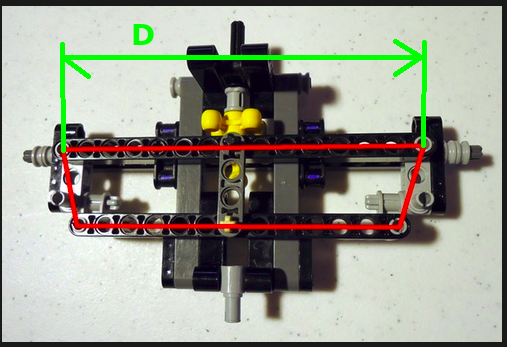
\includegraphics[width=\textwidth]{coll.png}
    \caption{Физический смысл длины $D$.}
    \label{img_coll}
\end{figure}
